\documentclass{article}
\usepackage{graphicx}
\graphicspath{{./figs/}}{}
\usepackage{listings}
\title{
HLS-Assignment 5 B
}
\begin{document}
\maketitle
\hfill \textbf{Sampath Govardhan} \\
\null \hfill \textbf{FWC22071}\\

\section{Problem Statement}
\begin{lstlisting}
Implement a DUT that takes 4 inputs in 4 clock cycles and then saves all the 
inputs in a BRAM (The BRAM should be contained within the DUT) at a single 
address. At the same time, it also gives out all the 4 inputs as a single 
bundle output in the same clock cycle when it receives the final input. The 
BRAM index will overflow after the BRAM is full and it should overwrite the 
old values as more inputs keep coming in.

\end{lstlisting}
\vspace{3cm}

\section{Design Code}
\begin{lstlisting}
#include"hls_stream.h"
#include "ap_int.h"
//#include "ap_axi_sdata.h"
using namespace std;

struct bundle{
	ap_uint<8> data[4];
};

void a5b(hls::stream<bundle> &in, hls::stream<bundle> &out){
bundle input=in.read();

bundle output={0,0,0,0};
ap_uint<8> bram[8];
#pragma HLS RESOURCE variable=bram core=RAM_1P_BRAM
#pragma HLS ARRAY_RESHAPE variable=bram cyclic factor=4 dim=1
ap_uint<3> c=0,add=0;
int ind=0;

for (int i=0;i<4;i++){

	if (c<8){
	bram[add]=input.data[ind];
	c=c+1;
	add=add+1;
	ind=ind+1;

	if (c==4){
	output.data[0]=bram[0];
	output.data[1]=bram[1];
	output.data[2]=bram[2];
	output.data[3]=bram[3];
	}
	}
	else{
	c=0;
	add=0;
	}
	}
	out.write(output);
	}


\end{lstlisting}
\vspace{5cm}


\section{Test Bench Code}
\begin{lstlisting}
#include<hls_stream.h>
#include <ap_int.h>
#include<iostream>
#include <fstream>
using namespace std;

struct bundle{
	ap_uint<8> data[4];
};


void a5b(hls::stream<bundle> &in, hls::stream<bundle> &out);
int main(){
hls::stream<bundle> indata;
hls::stream<bundle> outdata;
bundle input;
ifstream in;
ofstream out_d;

in.open("in.dat");
out_d.open("out.dat");

int i,index=0;
bool fail=0;

while (in>>i && index<4){
input.data[index]=i;
index=index+1;
}
indata.write(input);
a5b(indata,outdata);
bundle output=outdata.read();
for (int j=0;j<4;j++){
out_d<<output.data[j]<<" ";
}
if (input.data[0]==output.data[0] && input.data[1]==output.data[1] &&
 input.data[2]==output.data[2] && input.data[3]==output.data[3] ){
out_d<<"Pass"<<endl;
}
else{
out_d<<"Fail"<<endl;
fail++;
}
in.close();
out_d.close();
if (fail==0){
cout<<"ALL THE TEST CASES ARE PASSED!"<<endl;
}
else{
cout<<"ERROR! ALL THE TEST CASES ARE NOT PASSED!"<<endl;
}}


\end{lstlisting}
\vspace{3cm}

\section{in.dat file}
\begin{lstlisting}
7 8 6 4


\end{lstlisting}
\vspace{3cm}
\section{out.dat file}
\begin{lstlisting}
7 8 6 4 Pass


\end{lstlisting}
\vspace{15cm}


\section{HLS Resource Consumption}
\vspace{3cm}
\begin{figure}[h]
    \centering
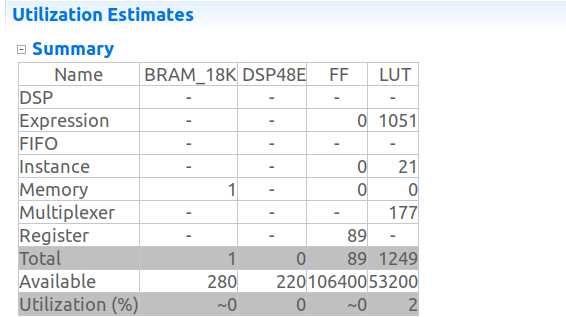
\includegraphics[width=\columnwidth]{1.png}
    \caption{Resource Consumption}
    \label{fig:my_label}
\end{figure}

\vspace{5cm}


\section{HLS Timing Report}
\vspace{1cm}
\begin{figure}[h]
    \centering
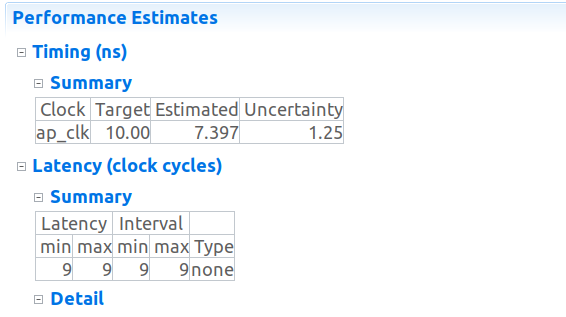
\includegraphics[width=\columnwidth]{figs/2.png}
    \caption{Timing Report}
    \label{fig:my_label}
\end{figure}

\vspace{10cm}


\section{Interfaces Report}
\vspace{1cm}
\begin{figure}[h]
    \centering
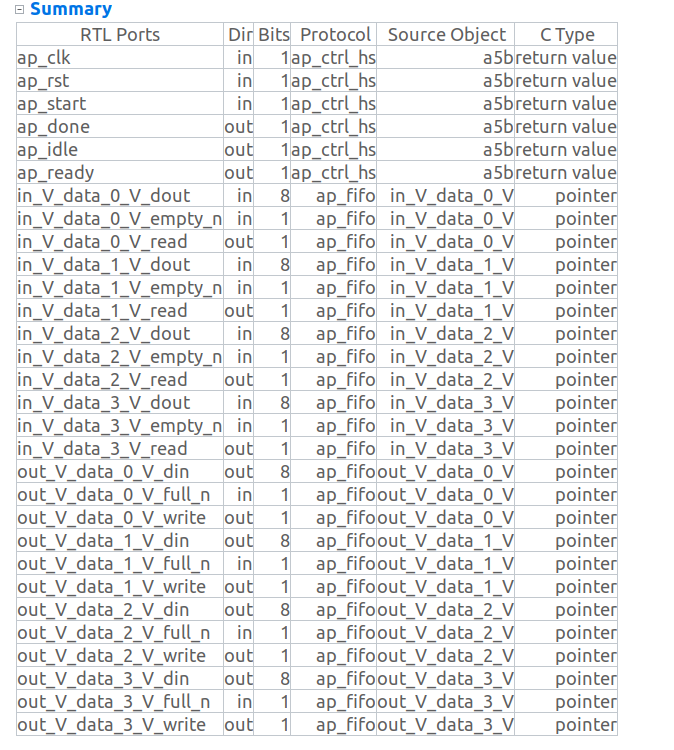
\includegraphics[width=\columnwidth]{figs/3.png}
    \caption{Interface Summmary}
    \label{fig:my_label}
\end{figure}
\vspace{5cm}

\section{C/RTL Cosimulation Output}
\begin{lstlisting}
Starting C/RTL cosimulation ...
/tools/Xilinx/Vivado/2018.3/bin/vivado_hls /home/sam-admin/git/Training/HLS_Assignments/A5/5.2/codes/Assignment5b/solution1/cosim.tcl
INFO: [HLS 200-10] Running '/tools/Xilinx/Vivado/2018.3/bin/unwrapped/lnx64.o/vivado_hls'
INFO: [HLS 200-10] For user 'sam-admin' on host 'sampaths-lappie' (Linux_x86_64 version 5.19.0-38-generic) on Mon Apr 03 17:23:33 IST 2023
INFO: [HLS 200-10] On os Ubuntu 22.04.2 LTS
INFO: [HLS 200-10] In directory '/home/sam-admin/git/Training/HLS_Assignments/A5/5.2/codes'
INFO: [HLS 200-10] Opening project '/home/sam-admin/git/Training/HLS_Assignments/A5/5.2/codes/Assignment5b'.
INFO: [HLS 200-10] Opening solution '/home/sam-admin/git/Training/HLS_Assignments/A5/5.2/codes/Assignment5b/solution1'.
INFO: [SYN 201-201] Setting up clock 'default' with a period of 10ns.
INFO: [HLS 200-10] Setting target device to 'xc7z020clg484-1'
INFO: [COSIM 212-47] Using XSIM for RTL simulation.
INFO: [COSIM 212-14] Instrumenting C test bench ...
   Build using "/tools/Xilinx/Vivado/2018.3/tps/lnx64/gcc-6.2.0/bin/g++"
   Compiling a5b.cpp_pre.cpp.tb.cpp
   Compiling a5b_tb.cpp_pre.cpp.tb.cpp
   Compiling apatb_a5b.cpp
   Generating cosim.tv.exe
INFO: [COSIM 212-302] Starting C TB testing ... 
ALL THE TEST CASES ARE PASSED!
INFO: [COSIM 212-333] Generating C post check test bench ...
INFO: [COSIM 212-12] Generating RTL test bench ...
INFO: [COSIM 212-323] Starting verilog simulation. 
INFO: [COSIM 212-15] Starting XSIM ...
INFO: [XSIM 43-3496] Using init file passed via -initfile option "/tools/Xilinx/Vivado/2018.3/data/xsim/ip/xsim_ip.ini".
Vivado Simulator 2018.3
Copyright 1986-1999, 2001-2018 Xilinx, Inc. All Rights Reserved.
Running: /tools/Xilinx/Vivado/2018.3/bin/unwrapped/lnx64.o/xelab xil_defaultlib.apatb_a5b_top glbl -prj a5b.prj -L smartconnect_v1_0 -L axi_protocol_checker_v1_1_12 -L axi_protocol_checker_v1_1_13 -L axis_protocol_checker_v1_1_11 -L axis_protocol_checker_v1_1_12 -L xil_defaultlib -L unisims_ver -L xpm --initfile /tools/Xilinx/Vivado/2018.3/data/xsim/ip/xsim_ip.ini --lib ieee_proposed=./ieee_proposed -s a5b 
Multi-threading is on. Using 6 slave threads.
WARNING: [XSIM 43-3431] One or more environment variables have been detected which affect the operation of the C compiler. These are typically not set in standard installations and are not tested by Xilinx, however they may be appropriate for your system, so the flow will attempt to continue.  If errors occur, try running xelab with the "-mt off -v 1" switches to see more information from the C compiler. The following environment variables have been detected:
    LIBRARY_PATH
INFO: [VRFC 10-2263] Analyzing SystemVerilog file "/home/sam-admin/git/Training/HLS_Assignments/A5/5.2/codes/Assignment5b/solution1/sim/verilog/glbl.v" into library work
INFO: [VRFC 10-311] analyzing module glbl
INFO: [VRFC 10-2263] Analyzing SystemVerilog file "/home/sam-admin/git/Training/HLS_Assignments/A5/5.2/codes/Assignment5b/solution1/sim/verilog/a5b.autotb.v" into library xil_defaultlib
INFO: [VRFC 10-311] analyzing module apatb_a5b_top
INFO: [VRFC 10-2263] Analyzing SystemVerilog file "/home/sam-admin/git/Training/HLS_Assignments/A5/5.2/codes/Assignment5b/solution1/sim/verilog/AESL_autofifo_in_V_data_2_V.v" into library xil_defaultlib
INFO: [VRFC 10-311] analyzing module AESL_autofifo_in_V_data_2_V
INFO: [VRFC 10-2263] Analyzing SystemVerilog file "/home/sam-admin/git/Training/HLS_Assignments/A5/5.2/codes/Assignment5b/solution1/sim/verilog/AESL_autofifo_out_V_data_0_V.v" into library xil_defaultlib
INFO: [VRFC 10-311] analyzing module AESL_autofifo_out_V_data_0_V
INFO: [VRFC 10-2263] Analyzing SystemVerilog file "/home/sam-admin/git/Training/HLS_Assignments/A5/5.2/codes/Assignment5b/solution1/sim/verilog/a5b.v" into library xil_defaultlib
INFO: [VRFC 10-311] analyzing module a5b
INFO: [VRFC 10-2263] Analyzing SystemVerilog file "/home/sam-admin/git/Training/HLS_Assignments/A5/5.2/codes/Assignment5b/solution1/sim/verilog/AESL_autofifo_out_V_data_3_V.v" into library xil_defaultlib
INFO: [VRFC 10-311] analyzing module AESL_autofifo_out_V_data_3_V
INFO: [VRFC 10-2263] Analyzing SystemVerilog file "/home/sam-admin/git/Training/HLS_Assignments/A5/5.2/codes/Assignment5b/solution1/sim/verilog/a5b_mux_42_8_1_1.v" into library xil_defaultlib
INFO: [VRFC 10-311] analyzing module a5b_mux_42_8_1_1
INFO: [VRFC 10-2263] Analyzing SystemVerilog file "/home/sam-admin/git/Training/HLS_Assignments/A5/5.2/codes/Assignment5b/solution1/sim/verilog/AESL_autofifo_out_V_data_2_V.v" into library xil_defaultlib
INFO: [VRFC 10-311] analyzing module AESL_autofifo_out_V_data_2_V
INFO: [VRFC 10-2263] Analyzing SystemVerilog file "/home/sam-admin/git/Training/HLS_Assignments/A5/5.2/codes/Assignment5b/solution1/sim/verilog/AESL_autofifo_in_V_data_3_V.v" into library xil_defaultlib
INFO: [VRFC 10-311] analyzing module AESL_autofifo_in_V_data_3_V
INFO: [VRFC 10-2263] Analyzing SystemVerilog file "/home/sam-admin/git/Training/HLS_Assignments/A5/5.2/codes/Assignment5b/solution1/sim/verilog/a5b_bram_V.v" into library xil_defaultlib
INFO: [VRFC 10-311] analyzing module a5b_bram_V_ram
INFO: [VRFC 10-311] analyzing module a5b_bram_V
INFO: [VRFC 10-2263] Analyzing SystemVerilog file "/home/sam-admin/git/Training/HLS_Assignments/A5/5.2/codes/Assignment5b/solution1/sim/verilog/AESL_autofifo_in_V_data_1_V.v" into library xil_defaultlib
INFO: [VRFC 10-311] analyzing module AESL_autofifo_in_V_data_1_V
INFO: [VRFC 10-2263] Analyzing SystemVerilog file "/home/sam-admin/git/Training/HLS_Assignments/A5/5.2/codes/Assignment5b/solution1/sim/verilog/AESL_autofifo_out_V_data_1_V.v" into library xil_defaultlib
INFO: [VRFC 10-311] analyzing module AESL_autofifo_out_V_data_1_V
INFO: [VRFC 10-2263] Analyzing SystemVerilog file "/home/sam-admin/git/Training/HLS_Assignments/A5/5.2/codes/Assignment5b/solution1/sim/verilog/AESL_autofifo_in_V_data_0_V.v" into library xil_defaultlib
INFO: [VRFC 10-311] analyzing module AESL_autofifo_in_V_data_0_V
Starting static elaboration
Completed static elaboration
Starting simulation data flow analysis
Completed simulation data flow analysis
Time Resolution for simulation is 1ps
Compiling module xil_defaultlib.a5b_bram_V_ram_default
Compiling module xil_defaultlib.a5b_bram_V(DataWidth=32,AddressR...
Compiling module xil_defaultlib.a5b_mux_42_8_1_1(ID=1,din0_WIDTH...
Compiling module xil_defaultlib.a5b
Compiling module xil_defaultlib.AESL_autofifo_in_V_data_0_V
Compiling module xil_defaultlib.AESL_autofifo_in_V_data_1_V
Compiling module xil_defaultlib.AESL_autofifo_in_V_data_2_V
Compiling module xil_defaultlib.AESL_autofifo_in_V_data_3_V
Compiling module xil_defaultlib.AESL_autofifo_out_V_data_0_V
Compiling module xil_defaultlib.AESL_autofifo_out_V_data_1_V
Compiling module xil_defaultlib.AESL_autofifo_out_V_data_2_V
Compiling module xil_defaultlib.AESL_autofifo_out_V_data_3_V
Compiling module xil_defaultlib.apatb_a5b_top
Compiling module work.glbl
Built simulation snapshot a5b


****** Webtalk v2018.3 (64-bit)
  **** SW Build 2405991 on Thu Dec  6 23:36:41 MST 2018
  **** IP Build 2404404 on Fri Dec  7 01:43:56 MST 2018
    ** Copyright 1986-2018 Xilinx, Inc. All Rights Reserved.


source /home/sam-admin/git/Training/HLS_Assignments/A5/5.2/codes/Assignment5b/solution1/sim/verilog/xsim.dir/a5b/webtalk/xsim_webtalk.tcl -notrace
INFO: [Common 17-206] Exiting Webtalk at Mon Apr  3 17:24:15 2023...


****** xsim v2018.3 (64-bit)
  **** SW Build 2405991 on Thu Dec  6 23:36:41 MST 2018
  **** IP Build 2404404 on Fri Dec  7 01:43:56 MST 2018
    ** Copyright 1986-2018 Xilinx, Inc. All Rights Reserved.


source xsim.dir/a5b/xsim_script.tcl
# xsim {a5b} -autoloadwcfg -tclbatch {a5b.tcl}
Vivado Simulator 2018.3
Time resolution is 1 ps
source a5b.tcl
## run all
////////////////////////////////////////////////////////////////////////////////////
// Inter-Transaction Progress: Completed Transaction / Total Transaction
// Intra-Transaction Progress: Measured Latency / Latency Estimation * 100%
//
// RTL Simulation : "Inter-Transaction Progress" ["Intra-Transaction Progress"] @ "Simulation Time"
////////////////////////////////////////////////////////////////////////////////////
// RTL Simulation : 0 / 1 [0.00%] @ "125000"
// RTL Simulation : 1 / 1 [100.00%] @ "235000"
////////////////////////////////////////////////////////////////////////////////////
$finish called at time : 275 ns : File "/home/sam-admin/git/Training/HLS_Assignments/A5/5.2/codes/Assignment5b/solution1/sim/verilog/a5b.autotb.v" Line 607
## quit
INFO: [Common 17-206] Exiting xsim at Mon Apr  3 17:24:23 2023...
INFO: [COSIM 212-316] Starting C post checking ...
ALL THE TEST CASES ARE PASSED!
INFO: [COSIM 212-1000] *** C/RTL co-simulation finished: PASS ***
INFO: [COSIM 212-211] II is measurable only when transaction number is greater than 1 in RTL simulation. Otherwise, they will be marked as all NA. If user wants to calculate them, please make sure there are at least 2 transactions in RTL simulation.
Finished C/RTL cosimulation.


\end{lstlisting}

\section{C/RTL Cosimulation Report}
\vspace{1cm}
\begin{figure}[h]
    \centering
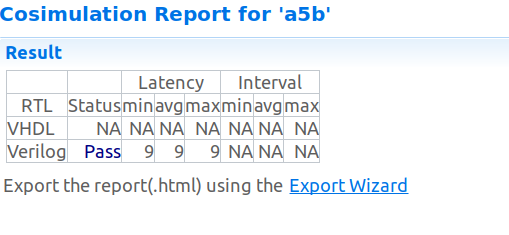
\includegraphics[width=\columnwidth]{figs/4.png}
    \caption{Cosimulation Report}
    \label{fig:my_label}
\end{figure}
\end{document}
